\documentclass[10pt,landscape,letterpaper]{article}
\usepackage[utf8]{inputenc}
\usepackage[T1]{fontenc}
%\usepackage[LY1,T1]{fontenc}
%\usepackage{frutigernext}
%\usepackage[lf,minionint]{MinionPro}
\usepackage{tikz}
\usetikzlibrary{shapes,positioning,arrows,fit,calc,graphs,graphs.standard}
\usepackage[nosf]{kpfonts}
\usepackage[t1]{sourcesanspro}
\usepackage{multicol}
\usepackage{wrapfig}
\usepackage[top=0mm,bottom=1mm,left=0mm,right=1mm]{geometry}
\usepackage[framemethod=tikz]{mdframed}
\usepackage{microtype}
\usepackage{pdfpages}
\usepackage{enumitem}

\let\bar\overline
\let\vec\mathbf

\setlist[itemize]{leftmargin=4mm}
\setlist[enumerate]{leftmargin=4mm}

\newcommand{\alert}[1]{\textbf{\color{red} #1}}

\definecolor{myblue}{cmyk}{1,.72,0,.38}

\def\firstcircle{(0,0) circle (1.5cm)}
\def\secondcircle{(0:2cm) circle (1.5cm)}

\colorlet{circle edge}{myblue}
\colorlet{circle area}{myblue!5}

\tikzset{filled/.style={fill=circle area, draw=circle edge, thick},
    outline/.style={draw=circle edge, thick}}

\pgfdeclarelayer{background}
\pgfsetlayers{background,main}

\everymath\expandafter{\the\everymath \color{myblue}}
\everydisplay\expandafter{\the\everydisplay \color{myblue}}

\renewcommand{\baselinestretch}{.8}
\pagestyle{empty}

\global\mdfdefinestyle{header}{%
linecolor=gray,linewidth=1pt,%
leftmargin=0mm,rightmargin=0mm,skipbelow=0mm,skipabove=0mm,
}

\newcommand{\header}{
\begin{mdframed}[style=header]
\footnotesize
\sffamily
Cheatsheet MEAM 620\\
fclad@seas.upenn.edu,~Pag.~\thepage~of~2
\end{mdframed}
}

\makeatletter % Author: https://tex.stackexchange.com/questions/218587/how-to-set-one-header-for-each-page-using-multicols
\renewcommand{\section}{\@startsection{section}{1}{0mm}%
                                {.2ex}%
                                {.2ex}%x
                                {\color{myblue}\sffamily\small\bfseries}}
\renewcommand{\subsection}{\@startsection{subsection}{1}{0mm}%
                                {.2ex}%
                                {.2ex}%x
                                {\sffamily\bfseries}}



\def\multi@column@out{%
   \ifnum\outputpenalty <-\@M
   \speci@ls \else
   \ifvoid\colbreak@box\else
     \mult@info\@ne{Re-adding forced
               break(s) for splitting}%
     \setbox\@cclv\vbox{%
        \unvbox\colbreak@box
        \penalty-\@Mv\unvbox\@cclv}%
   \fi
   \splittopskip\topskip
   \splitmaxdepth\maxdepth
   \dimen@\@colroom
   \divide\skip\footins\col@number
   \ifvoid\footins \else
      \leave@mult@footins
   \fi
   \let\ifshr@kingsaved\ifshr@king
   \ifvbox \@kludgeins
     \advance \dimen@ -\ht\@kludgeins
     \ifdim \wd\@kludgeins>\z@
        \shr@nkingtrue
     \fi
   \fi
   \process@cols\mult@gfirstbox{%
%%%%% START CHANGE
\ifnum\count@=\numexpr\mult@rightbox+2\relax
          \setbox\count@\vsplit\@cclv to \dimexpr \dimen@-1cm\relax
\setbox\count@\vbox to \dimen@{\vbox to 1cm{\header}\unvbox\count@\vss}%
\else
      \setbox\count@\vsplit\@cclv to \dimen@
\fi
%%%%% END CHANGE
            \set@keptmarks
            \setbox\count@
                 \vbox to\dimen@
                  {\unvbox\count@
                   \remove@discardable@items
                   \ifshr@nking\vfill\fi}%
           }%
   \setbox\mult@rightbox
       \vsplit\@cclv to\dimen@
   \set@keptmarks
   \setbox\mult@rightbox\vbox to\dimen@
          {\unvbox\mult@rightbox
           \remove@discardable@items
           \ifshr@nking\vfill\fi}%
   \let\ifshr@king\ifshr@kingsaved
   \ifvoid\@cclv \else
       \unvbox\@cclv
       \ifnum\outputpenalty=\@M
       \else
          \penalty\outputpenalty
       \fi
       \ifvoid\footins\else
         \PackageWarning{multicol}%
          {I moved some lines to
           the next page.\MessageBreak
           Footnotes on page
           \thepage\space might be wrong}%
       \fi
       \ifnum \c@tracingmulticols>\thr@@
                    \hrule\allowbreak \fi
   \fi
   \ifx\@empty\kept@firstmark
      \let\firstmark\kept@topmark
      \let\botmark\kept@topmark
   \else
      \let\firstmark\kept@firstmark
      \let\botmark\kept@botmark
   \fi
   \let\topmark\kept@topmark
   \mult@info\tw@
        {Use kept top mark:\MessageBreak
          \meaning\kept@topmark
         \MessageBreak
         Use kept first mark:\MessageBreak
          \meaning\kept@firstmark
        \MessageBreak
         Use kept bot mark:\MessageBreak
          \meaning\kept@botmark
        \MessageBreak
         Produce first mark:\MessageBreak
          \meaning\firstmark
        \MessageBreak
        Produce bot mark:\MessageBreak
          \meaning\botmark
         \@gobbletwo}%
   \setbox\@cclv\vbox{\unvbox\partial@page
                      \page@sofar}%
   \@makecol\@outputpage
     \global\let\kept@topmark\botmark
     \global\let\kept@firstmark\@empty
     \global\let\kept@botmark\@empty
     \mult@info\tw@
        {(Re)Init top mark:\MessageBreak
         \meaning\kept@topmark
         \@gobbletwo}%
   \global\@colroom\@colht
   \global \@mparbottom \z@
   \process@deferreds
   \@whilesw\if@fcolmade\fi{\@outputpage
      \global\@colroom\@colht
      \process@deferreds}%
   \mult@info\@ne
     {Colroom:\MessageBreak
      \the\@colht\space
              after float space removed
              = \the\@colroom \@gobble}%
    \set@mult@vsize \global
  \fi}

\makeatother
\setlength{\parindent}{0pt}


\begin{document}
%\footnotesize
\small
\begin{multicols*}{5}
\section{Kinematics Equations}
\subsection*{Skew-symmetric matrix}
$[a]_\times = \begin{pmatrix}
  0 & -a_3 & a_2 \\ 
  a_3 & 0 -a_1 \\
  -a_2 & a_1 & 0
\end{pmatrix}$

\subsection*{Angular velocities}
$\hat\omega_b = R^T \dot{R}$ \\
$\hat\omega_s = \dot{R}R^T$ \\
where $R$ has to be in inertial frame ($^W R_C$).

% ---------
% \newline

\section{CV basics}
\subsection*{Pinhole model}
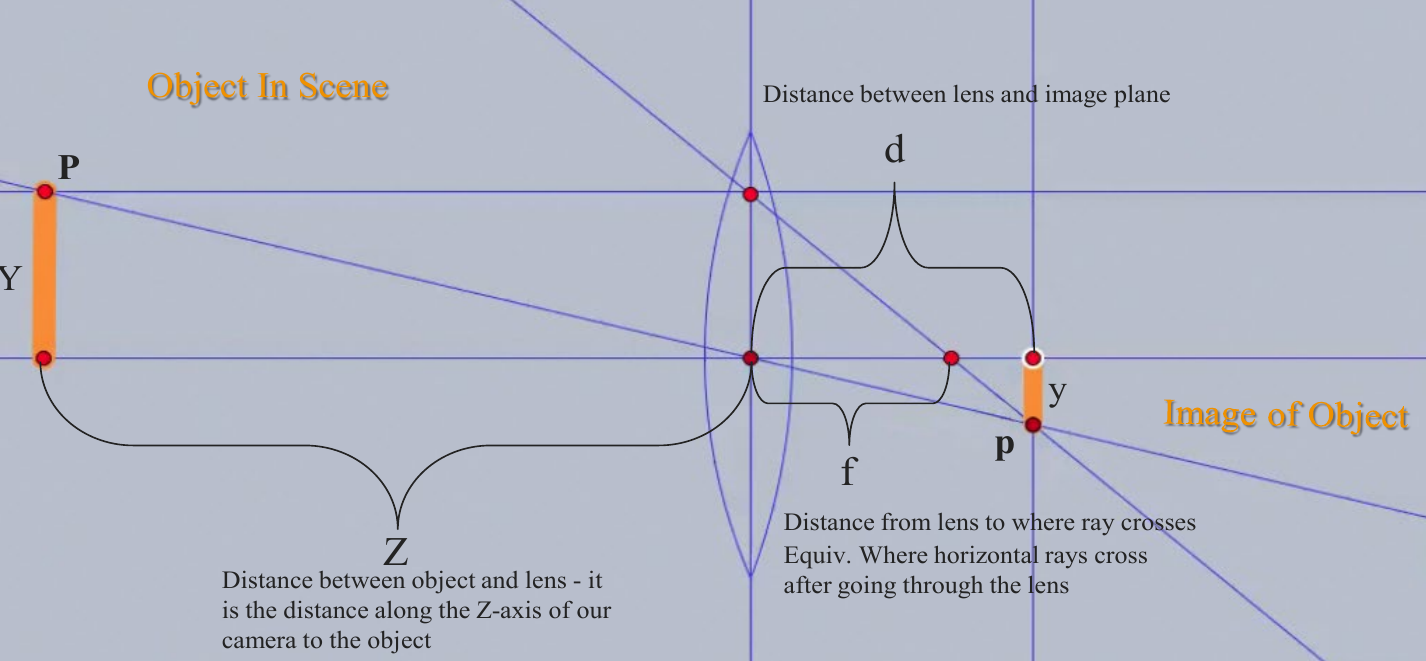
\includegraphics[width=\linewidth]{Images/Pinhole.png}
$1/f = 1/Z + 1/d$ \\
$Y/Z = y/d \Rightarrow y = d Y/Z$\\
Problem: d changes depending where the object is in the scene. Hence:
$y \approx f Y/Z$\\
\alert{Only valid if $Z >> d$}

\subsection*{Calibration}
\begin{itemize}
  \item Find $f$.
  \item Radial distortion:\\
    $r = norm(x, y), x' = x( 1 + k_1 t + k_2 r^2
    + k_3 r^3$\\
    (and similar for y)
\end{itemize}

\subsection*{Projection Equation}
$\begin{pmatrix} u\\ v\\ w\end{pmatrix} \sim
S \begin{pmatrix}r_1 & r_2 & r_3 & t \end{pmatrix}
\begin{pmatrix} X_w \\ Y_w \\ Z_w \\ 1\end{pmatrix}$ \\
$\begin{pmatrix} u\\ v\\ w\end{pmatrix} \sim
S \begin{pmatrix} ^C R_W & ^C T_W \end{pmatrix}
\begin{pmatrix} X_w \\ Y_w \\ Z_w \\ 1\end{pmatrix}$ \\
where $S = [f 0 x_0; 0 f y_0; 0 0 1]$\\
\includegraphics[width=\linewidth]{Images/projection.png}

\alert{$t$ is the distance from the camera to the world coordinate
system in camera coordinates}

\subsection*{Projective Geometry}
\begin{itemize}
  \item 
\end{itemize}


\section{Homographies}
\subsection*{Constant plane in X, Y, Z}
Eg. for $X = h$:  $H = \begin{pmatrix}
  r_2 & r_3 & h r_1 + t
\end{pmatrix}$ 

\subsection*{Plane constraint}
Eg: $A X_w + B Y_w + C Z_w = 1$
\begin{itemize}
  \item Substitute the 1 in the last position. Expand.
  \item Replace $Z_w = 1/C (A X_w + B Y_w)$
\end{itemize}

\section{PnP}
\begin{itemize}
  \item \textbf{Got:} 2D-3D correspondences
  \item \textbf{Want:} $T, R$ between camera and world coordinate
    system.
\end{itemize}

\textbf{Solutions}
\begin{itemize}
  \item Linear hack (hw 3)\\
    $\lambda_i \begin{pmatrix} x_i \\ y_i \\ 1 \end{pmatrix} = R
    \begin{pmatrix}X_i \\ Y_i \\ Z_i \end{pmatrix} + T$\\
    Expand the matrices.
    Solve for $\lambda_i$, and get two equations per point. \alert{We
    need at least 6 points}.
  \item Non-linear optimization
  \item P3P
\end{itemize}

\subsection*{P3P}
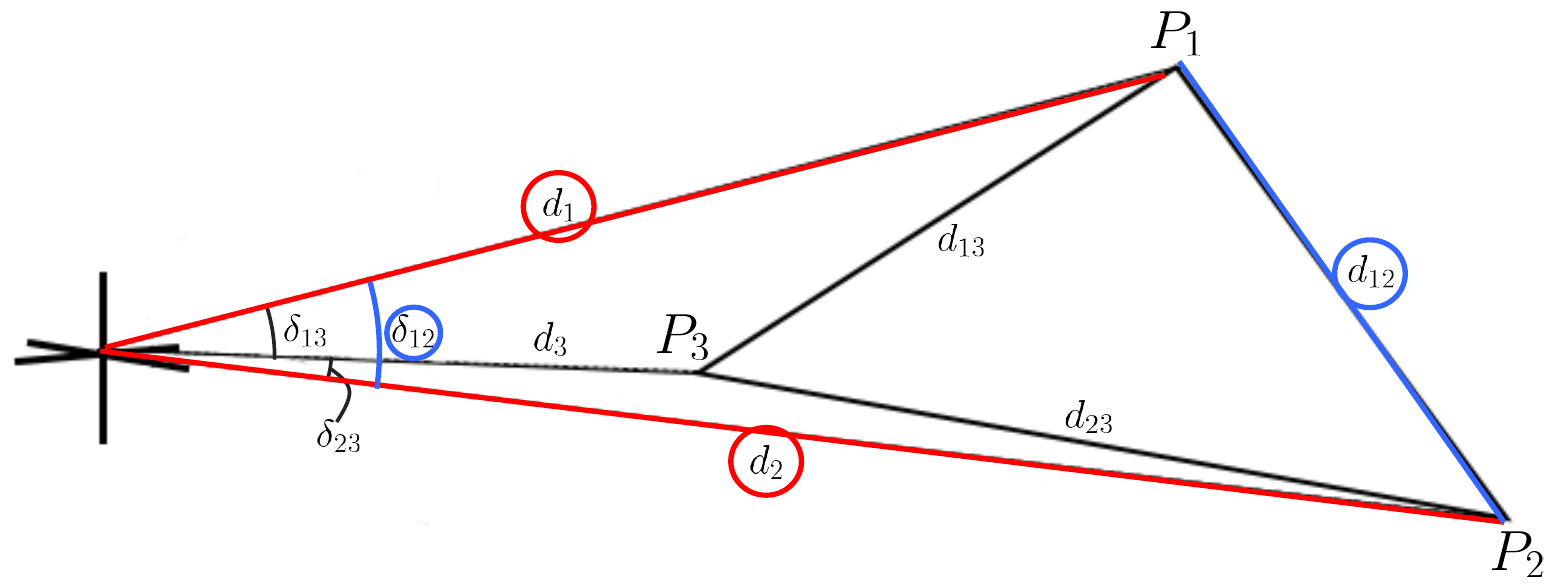
\includegraphics[width=\linewidth]{Images/P3P.png}
Simple formulation:\\
$d_i^2 + d_j^2 - 2 d_i d_j \cos(\delta_{ij}) = d_{ij}^2$\\
\alert{Use this for simple problems!}

Complex formulation: we use $d_2 = u d_1$, $d_3 = v d_1$, then:\\
$d_{13}^2 (u^2 + v^2 - 2 u v \cos(\delta_{23}) \\= 
d_{23}^2(1+v^2 - 2 v cos(\delta_{13}))$\\
$d_{12}^2 (1 + v^2 - 2v \cos(\delta_{13})) \\=
d_{13}^2 (1 + u^2 - 2u \cos(\delta_{12}))$
\begin{enumerate}
  \item Solve $u^2$ in 1.
  \item Insert $u^2$ back into 2.
  \item Solve $u$, leaving tems in $v$ and $v^2$.
  \item Insert $u$ back into 1. Quartic polynomial in $v$.
    \alert{At most 4 solutions}.
\end{enumerate}

\alert{To find the angles, we can use the dot product of the rays.}
Each pixel on the camera image denotes a direction. Using camera K matrix, you can find the vector in the camera frame. Using inner products give the angle cosines.

After solving P3P, we have to use procrustes to find $R$ and $T$.

\section{Procrustes (3D-3D registration)}
\begin{itemize}
  \item \textbf{Got:} two set of 3D points
  \item \textbf{Want:} $R, T$ such that\\
    $\min_{R,T} \sum |A_i - R B_i +T|^2$
\end{itemize}

\subsection*{Procrustes solution:}
\begin{enumerate}
  \item $\bar{P} = \dfrac{1}{N} \sum P_i$,
    $bar{P'} = \dfrac{1}{N} \sum P_i'$\\
  \item $Z = \sum(P_i - \bar{P})(P_i' - \bar{P'})^T = U S V^T$
  \item Rectify $R$ using the same trick we use in pose estimation.
  \item $T = \bar{P'} - R \bar{P}$
\end{enumerate}

% Solving Procrustes (by expanding the previous equation):\\
% $= 2 \left( \sum R P_i - P_i' \right)^T T + N T^T T -\\
% 2 \sum(P_i'^T R P_i) + \sum P_i^T P_i + \sum P_i'^T P_i'$
% 
% Derivate w.r.t. $T$ to find $T$\\
% $\Rightarrow T = \dfrac{1}{N} \sum P_i' - R P_i\\
% = \bar{P'} - R \bar{P}$\\
% The translation is the difference between the centroids.
% 
% Substract the centroids to the points to get rid of the translation
% points:\\
% $\tilde{P_i} = P_i - \bar{P}$ , $\tilde{P_i'} = P_i' - \bar{P'}$\\
% $argmin_{R \in SO(3)} \sum |R \tilde{P_i} - \tilde{P_i'}|$
% 
% Which yields:
% 
% $argmax_{R \in SO(3)} \sum \tilde{P_i'}^T R \tilde{P_i} = tr(RZ)$\\
% $ = tr (R U S V^T) = tr((V^T R U) S) = tr(QS)$
% 
% We make $Q$ identity to maximize, and we have.



\section{Optical Flow}
$\vec{p} = \dfrac{1}{Z} A(\vec{p}) V + B(\vec{p}) \Omega$\\
where \\
$A(\vec{p}) = \begin{pmatrix}
  -1 & 0 & p_x \\ 0 & -1 & p_y
\end{pmatrix}$\\
$B(\vec{p}) = \begin{pmatrix}
  -p_x p_y & -(p_x^2 +1) & p_y \\
  1 + p_y^2 & -p_x p_y & -p_x
\end{pmatrix}$\\
$V$: velocity in \alert{inertial frame}\\
$\Omega$: ang velocity in \alert{intertial frame}\\
$\vec{p}$: 2D point in the image \\
$\dot{\vec{p}}$: 2D velocity in the image

How to find this?\\
$\vec{p} = \vec{P}/Z$\\
$\dot{\vec{p}} = \dot{\vec{P}}/Z - \dot{Z}/Z \vec{p}$\\
$\dot{Z} = e_3^T \dot{\vec{P}}$\\
$\dot{\vec{P}} = - \vec{V} - \vec{\Omega} \times \vec{P}$\\
$=1/Z ( \vec{p} e_3^T - I) \vec{V} + (I - \vec{p} e_3^T)[p]_\times
\vec{\Omega}$

\textbf{Cases}
\begin{itemize}
  \item Known depth:\\
    $\vec{V}, \vec{\Omega} = argmin_{\vec{V}, \vec{\Omega}}\\
    \sum |\begin{pmatrix} \dfrac{1}{Z_i} A(\vec{p}_i) &
    B(\vec{p}_i)\end{pmatrix} 
    \begin{pmatrix}
      \vec{V}\\\vec{\Omega}
    \end{pmatrix} - \dot{\vec{p}}_i|^2$
  \item No translational vel:\\
    \alert{Useful when the drone is flying very high, or if we want to
    track the stars}.\\
    $\vec{\Sigma}^* = argmin_{\vec{\Sigma}}
    \sum |B(\vec{p}_i \vec{\Sigma} - \dot{\vec{p}}_i|^2$
  \item No angular vel:\\
    \alert{We use the cross product trick to eliminate $Z_i$}
    $\dot{\vec{p}} = \dfrac{1}{Z_i} A(\vec{p}) \vec{V}$\\
    $[\dot{\vec{p}}]_{\times} A(\vec{p}) \vec{V} = 0$\\
    And we can do SVD here.
  \item Everything unknown. Difficult problem.
\end{itemize}

\subsection*{Optical flow as a local search}
Assumptions:
\begin{itemize}
  \item Brightness consistency
  \item Minimal geometric deformations
  \item Minimal patch displacement
  \item Patch is sufficiently interesting
  \item Wall is not ''white''.
\end{itemize}
Barberpole issue: we cannot see if it moves in a specific direction.

\textbf{Finding features}(SURF) -> \textbf{Track them} (KLT)

\section{Structure from Motion (SFM)}
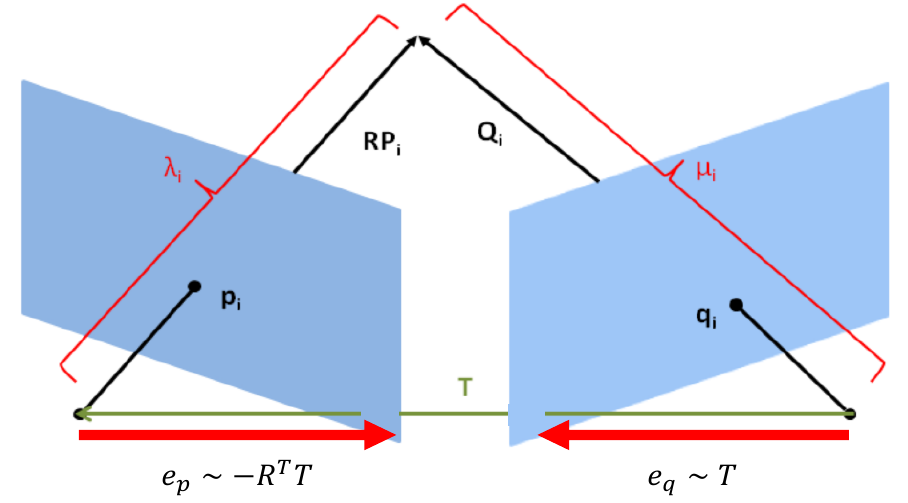
\includegraphics[width=\linewidth]{Images/SFM.png}
\begin{itemize}
  \item \textbf{Got:} 2D-2D correspondences between two views $p$, $q$.
  \item \textbf{Want:} $T, R$ between two views.
\end{itemize}
$\mu q = R \lambda p + T$\\
$T$ is here in the coordinates of $q$.\\
$DOF = 6$ (3 translation, 3 rotation), but 
we can only find the translation up to a scale. Finally, $DOF = 5$.

\subsection*{Epipolar constraint}
From the image, we see that the vectors $\mu q$, $T$ and $\lambda R p$
are coplanar. We can write the triple product:
$\mu q^T ( T \times \lambda R p) = 0$\\
$q^T ( T \times R p) = 0$\\
$q^T \hat{T} R p = 0$

The planes spanned by $T$, $\lambda q$ and $\mu p$ is called epipolar
plane (cross product vanishes).

\alert{Whe we cannot recover the scale?}\\
In the previous equation, scaling $q$ or $p$ will not violate the
constraint. Therefore, we can obtain the translation up to a scale.

\subsection*{Essential Matrix}
$q^T E p = 0$, where $E = \hat{T} R$

\subsection*{Fundamental Matrix}
If our points are not calibrated, we have to calibrate them:\\
$F = K^{-T} \hat{T} R K'^-1$

\subsection*{Epipolar Line}
In $p$-plane, line with coefficients $E^T q$.

All epipolar lines go through the epipole $e_p$:\\
$E e_p = \hat{T} R (-R^T T) = \hat{T}T = T \times T = 0$

\subsection*{Essential Matrix Calculation}
$E = \begin{pmatrix}e_1 & e_2 & e_3 \end{pmatrix}$\\
$q^T \begin{pmatrix}e_1 & e_2 & e_3 \end{pmatrix}
\begin{pmatrix}p_x \\ p_y \\ p_z \end{pmatrix}$ \\
$= \begin{pmatrix}p_x q^T & p_y q^T&p_z q^T \end{pmatrix}
\begin{pmatrix}e_1 \\ e_2 \\ e_3 \end{pmatrix}$\\
8-point algorithm\\
$\vec{a} = \begin{pmatrix}p_x q^T & p_y q^T&p_z q^T \end{pmatrix}$
$\begin{pmatrix} a_1^T \\ a_2^T \\ \vdots \\ a_n^T \end{pmatrix} E' =
0$\\
and we do SVD. Practically: \\
$E = U \text{diag}\left(\dfrac{\sigma_1 + \sigma_2}{2}, \dfrac{\sigma_1
+ \sigma_2}{2}, 0 \right) V^T$j

Other options for estimation:
\begin{itemize}
  \item 5 point algorithm. Quite complex.
  \item 7 point algorithm. Easier, don't need to do full estimation.
\end{itemize}

\alert{Always do RANSAC when estimating E, because we can have bad
points matches}

\subsection*{Essential matrix properties}
$E = \hat{T} R \Rightarrow E E^T = \hat{T} \hat{T}^T$ 
$=T T^T - T^T T I$
$=\begin{pmatrix} 
  t_x^2 & t_x t_y & t_x t_z \\
  t_x t_y & t_y^2 & t_y t_z \\
  t_x t_z & t_y t_z & t_z^2
\end{pmatrix} - |T|^2 I$\\
If we solve $det(E E^T - \lambda I) = 0$, we found two eigenvalues
$|T|^2$.\\
To be essential, $E$ should have $\sigma_1 = \sigma_2 > 0$ and $\sigma_3
= 0$

\subsection*{Essential matrix decomposition}
Useful properties: \\
$\hat{Q a} = Q \hat{a} Q^T$\\
$\begin{pmatrix}
  1 & 0 & 0 \\ 0 & 1 & 0 \\ 0& 0& 0
\end{pmatrix} =\hat{T}^T_z R_{z, \pi/2}$ \\
Therefore we can write
$E = \sigma U
\begin{pmatrix}
  1 & 0 & 0 \\ 0 & 1 & 0 \\ 0& 0& 0
\end{pmatrix} V^T$\\
$=\sigma \underbrace{U \hat{T}^T_z}_{\text{antisymmetric}}
\underbrace{R_z V^T}_{\text{orthogonal}}$

Two $R$:
\begin{itemize}
  \item $R_1 = U R^T_{z, \pi/2} V^T$
  \item $R_2 = U R^T_{z, -\pi/2} V^T$
\end{itemize}
Two $\hat{T}$:
\begin{itemize}
  \item $T_1 = U R^T_{z, \pi/2} \Sigma U^T$
  \item $T_2 = U R^T_{z, -\pi/2} \Sigma U^T$
\end{itemize}

Where\\
$T_{z, \pi/2} = \begin{pmatrix} 
  0 & 1 & 0 \\ -1 & 0 & 0\\ 0 & 0 & 0
\end{pmatrix}$

Finally, disembiguate with $\lambda q = \mu R p + T$ such that $\lambda,
\mu > 0$


\subsection*{Triangulation}
\begin{itemize}
  \item \textbf{Got:} $T, R$ and 2D correspondences in two images.
  \item \textbf{Want:} Depth of points in each camera $\mu_i$, $\lambda_i$.
\end{itemize}

We set the translation to $|T| = 1$
$\underbrace{\begin{pmatrix}q_i & -R p_i\end{pmatrix}}_{3\times2}
\underbrace{\begin{pmatrix} \mu_i \\\lambda_i \end{pmatrix}}_{2\times1} =
\underbrace{T}_{3 \times 1}$\\
3 eqs with 2 unknowns, solve with pseudoinverse

\subsection*{Tips and Tricks}
\begin{itemize}
  \item $R = I$, the epipolar constraint is\\
    $q^T ( T \times p) = 0$ or $(q \times p)^T T = 0$.\\
    We need 2 points to solve the problem (up to a scale).
  \item Pure translation essential matrix: we can recognize if it is
    skew symmetric. If $E$ is antisymmetric, that means that $R = I$!
\end{itemize}

\section{RANSAC}
\subsection*{Hough transform}
Parametrize points $\rightarrow$ voting system.

Issues:
\begin{itemize}
  \item Memory grows exponentially in parameter space.
  \item Need bounds in parameter space
\end{itemize}

\subsection*{Sample consensus}
Do it for all the points, count the one that has the most inliers.
Problem: a lot of combinations.

\subsection*{RANSAC inliers}
$k = \dfrac{\log(1 - p_{success}}{\log(1 - \epsilon^M)}$\\
where $k$: iterations, $p_{success}$: target success probability,
$\epsilon$: inlier proportion in set, $M$: minimum number of points for
model.


\section{VO}
\begin{itemize}
  \item \textbf{SFM}: 3D reconstruction and pose estimation from image sets.
  \item \textbf{VO}: focus on estimation and local consistency.
  \item \textbf{SLAM}: focus on gloval consistence. VSLAM = visual odometry +
    loop closure + graph optimization.
\end{itemize}

\alert{Why VO?}
No wheel slip.
More accurate trajectory estimates.
GPS-denied environments.

\alert{Why not?}
Low illumination.
A lot of moving objects.
Not texture.

\alert{Solution:} complementary sensor suite. Camera + IMU.

\section{Kalman Filter}
\subsection*{Assumptions}
\begin{itemize}
  \item $p(x_0) \sim N(\mu_0, \Sigma_0)$
  \item $p(x_t|x_{t-1}, u_t)$ linear, AGWN.
    \begin{itemize}
      \item $x_t = A_t x_{t-1} + B_t u_t + n_t$
      \item $n_t \sim N(0, Q_t)$
      \item $x_t, n_t \in R^n$, $u_t \in R^m$, 
        $A_t, Q_t \in R^{n\times n}$, $B_t \in R^{n \times m}$
    \end{itemize}
  \item $p(z_t|x_t)$ linear, AGWN
    \begin{itemize}
      \item $z_t = C_t x_t + v_t$
      \item $v_t \sim N(0, R_t)$
      \item $z_t, v_t \in R^p$, $C_t \in R^{p \times n}$, $R_t \in R^{p
        \times p}$
    \end{itemize}
\end{itemize}

\subsection*{Equations}
\textbf{Prediction}: uses input $u_t$ and $Q_t$:\\
$\bar{\Sigma}_t$\\
$\bar{\mu_t} = A \mu_{t-1} + B u_t$ \\
$\bar{\Sigma_t} = A \Sigma_{t-1} A^T + Q$

\textbf{Where does this come?}
\begin{itemize}
  \item Sum of gausians: $z = x + y$ is also a gaussian with $\mu_z =
    \mu_x + \mu_y$, $\Sigma_z = \Sigma_x + \Sigma_y$.
  \item Affine transformations: \\$X \sim N(\mu_X, \Sigma_X)$, $Y= AX +
    b$, then $Y \sim N(\mu_Y, \Sigma_Y)$, $\mu_Y = A \mu_X + b$,\\
    $\Sigma_Y = A \Sigma_X A^T$.
\end{itemize}

\textbf{Update}: uses measurement $z_t$ and $R_t$:\\
$K_t = \bar{\Sigma}_t C^T (C \bar{\Sigma}_t C^T + R)^{-1}$ \\
$\mu_t = \bar{\mu}_t + K_t (\underbrace{z_t - C
\bar{\mu}_t}_{\text{Innovation}})$ \\
$\Sigma_t = \bar{\Sigma}_t - K_t C \bar{\Sigma}_t$

\textbf{Where does this come?}
\begin{itemize}
  \item 
  $Y = [X \, Z]^T$ multivariate Gaussian, $\mu = [\mu_X \, \mu_Z]^T$,\\
  $\Sigma = [\Sigma_{XX} \, \Sigma_{XZ}; \Sigma_{ZX} \, \Sigma_{ZZ}]$\\
  $p(X|Z) = P(X, Z)/P(Z)$ has \\
  $\mu_{X|Z} = \mu_X + \Sigma_{XZ} \Sigma_{ZZ}^{-1}(X - \mu_Z)$\\
  $\Sigma_{X|Z} = \Sigma_{XX} - \Sigma_{XZ} \Sigma_{ZZ}^{-1} \Sigma_{ZX}$
\item The best update without a measurement is $x_t = \bar{x}_t$. Then\\
  $\begin{pmatrix}x_t \\ z_t\end{pmatrix} = 
  \begin{pmatrix}I & 0\\ C & I\end{pmatrix}
  \begin{pmatrix}\bar{x}_t \\ v_t\end{pmatrix}$ \\
  With mean  $[\bar{\mu}_t \, C\bar{\mu}_t]^T$ and\\
  $ \Sigma = 
  \begin{pmatrix}
    I & 0 \\ C & I
  \end{pmatrix}
  \begin{pmatrix}
    \bar{\Sigma}_t & 0 \\ 0 & R
  \end{pmatrix}
  \begin{pmatrix}
    I & C^T \\ 0 & I
  \end{pmatrix}\\
  =
  \begin{pmatrix}
    \bar{\Sigma}_t & \bar{\Sigma}_t C^T \\
    C \bar{\Sigma}_t & C \bar{\Sigma}_t C^T + R
  \end{pmatrix}
  $
\end{itemize}

\subsection*{Kalman Gain}
Degree to which the measurement is incorporated ("trusted")
\begin{itemize}
  \item Perfect sensor: $R = 0$\\
    $K_t = C^{-1}$, $\mu_t = C^{-1} z_t$, $\Sigma_t = 0$
  \item Horrible sensor: $R \to \infty$\\
    $K_t \to 0$ $\mu_t \to \bar{\mu}_t$, $\Sigma_t \to \bar{\Sigma}_t$
\end{itemize}

\subsection*{Kalman Facts}
\begin{itemize}
  \item If dist. not gaussian, Kalman filter is the minimum variance
    linear estimator (noise must be uncorrelated with initial state
    $x_0$).
  \item \alert{Variance never increases due to receiving a measurement}.
  \item \alert{Variance update independent of the measurement
    realization}.
  \item The Kalman filter permits individual update steps for each
    sensor as data becomes available.
\end{itemize}

\section{Extended Kalman Filter}
\begin{itemize}
  \item $p(x_0) \sim N(\mu_0, \Sigma_0)$
  \item $\dot{x}_t = f(x_t, u_t, n_t)$, $n_t\sim N(0, Q_t)$
  \item $z = h(x, v)$, $v_t \sim N(0, R_t)$
\end{itemize}

We use one-step Euler integration to discretize the system in the
interval $\tau = [t', t)$.

\subsection*{Prediction Linearization}
\textbf{Linearize dynamics around\\$x = \mu_{t-1}$, $u = u_t$, $n = 0$}\\
$f(x_t, u, n) \approx f(\mu_{t-1}, u_t, 0) +\\
\underbrace{\dfrac{\partial f}{\partial x}\Bigr|_{\substack{\mu_{t-1},
u_t}}}_{A_t}(x - \mu_{t-1}) + \underbrace{\dfrac{\partial f}{\partial u}\Bigr|_{\substack{\mu_{t-1},
u_t}}}_{B_t}(u - u_t) +\\
\underbrace{\dfrac{\partial f}{\partial n}\Bigr|_{\substack{\mu_{t-1},
u_t}}}_{U_t}(n - 0)
$\\

\textbf{One-step Euler integration}\\
$x_t \approx x_{t-1} + f(x_{t-1}, u_t, n_t) \delta t$\\
$x_t \approx x_{t-1} + (  f(\mu_{t-1}, u_t, 0) + \\
A_t (x_{t-1} - \mu_{t-1})  +  U_t n) \delta t$\\
$x_t \approx \underbrace{(I + A_t \delta t)}_{F_t} x_{t-1}
+ \underbrace{(U_t \delta_t)}_{V_t} n_t + \\
\underbrace{\left( f(\mu_{t-1}, u_t, 0) - ª_t \mu_{t-1}\right) \delta t}_{b_t}$
\begin{itemize}
  \item $\bar{\mu}_t = F_t \mu_{t-1} + b_t \\
    = \mu_{t-1} + \delta t f(\mu_{t-1}, u_t, 0)$
  \item $\bar{\Sigma}_t = F_t \Sigma_{t-1} F_t^T + V_t Q_t
    V_t^T$
\end{itemize}

\subsection*{Update Linearization}
\textbf{Linearize observation model around\\
$x = \bar{\mu}_t$, $v=0$}\\
$h(x, v) \approx h(\bar{\mu}_t, 0) + \\
\underbrace{\dfrac{\partial h}{\partial x}\Bigr|_{\substack{\bar{\mu}_t,
0}}}_{C_t}(x - \bar{\mu}_t) +
\underbrace{\dfrac{\partial h}{\partial v}\Bigr|_{\substack{\bar{\mu}_t,
0}}}_{W_t}(v - 0)$\\
$z_t \approx h(\bar{\mu_t}, 0) + C_t (x_t - \bar{\mu}_t) + W_t  v_t$\\
We define the matrix\\
$
\begin{pmatrix}
  x_t \\ z_t
\end{pmatrix} =
\begin{pmatrix}
  I & 0\\C_t & W_t
\end{pmatrix}
\begin{pmatrix}
  \bar{x}_t \\ z_t
\end{pmatrix} +
\begin{pmatrix}
  0 \\ h(\bar{\mu}_t, 0) - C_t \bar{\mu}_t
\end{pmatrix}
$
$
\Sigma =
\begin{pmatrix}
  \bar{\Sigma_t} & \bar{\Sigma}_t C_t^T\\
  C_t \bar{\Sigma}_t & C_t \bar{\Sigma}_t C_t^T + W_t R_t W_t^T
\end{pmatrix}
$

\begin{itemize}
  \item $\mu_t = \bar{\mu}_t + K_T(z_t - h(\bar{\mu}_t, 0))$
  \item $\Sigma_t = \bar{\Sigma}_t - K_t C_t \bar{\Sigma}_t$
  \item $K_t = \bar{\Sigma}_t C_t^T (C_t \bar{\Sigma}_t C_t^T + W_t R_t
    W_t^T)^{-1}$
\end{itemize}

\subsection*{Project Implementations}
Why choose sensors as inputs instead of observations?
\begin{itemize}
  \item Keeps state space and dimenstion of belief small.
  \item We might have very high confidence in the sensors (and very low
    confidence in our aerodynamical model).
\end{itemize}

\textbf{Model}\\
$\vec{\omega} = \begin{pmatrix} p & q & r\end{pmatrix}^T = \\
\begin{pmatrix}
  c \theta & 0 & -c \phi s \theta \\
  0 & 1 & s \phi \\
  s \theta & 0 & c \phi c \theta
\end{pmatrix}
\begin{pmatrix}
  \dot{\phi} & \dot{\theta} & \dot{\psi}
\end{pmatrix} = T(\vec{q}) \dot{\vec{q}}
$

\textbf{First Implementation}: gyro + VICON (linear vel)\\
$\vec{x} = \begin{pmatrix}\vec{p}   & \vec{q} & \vec{b}_g\end{pmatrix}^T$\\
$\vec{u} = \begin{pmatrix}\vec{v}_m & \vec{\omega}_m\end{pmatrix}^T$\\
with ($\vec{b}_g$ bias gyro)\\
$\vec{v}_m = \dot{\vec{p}}_m + \vec{n}_v$\\
$\vec{\omega}_m = \vec{\omega} + \vec{b}_g + \vec{n}_g$\\
$\dot{\vec{b}}_g = \vec{n}_{bg} \sim N(0, Q_g)$ (bias gyro drift)\\

$\dot{\vec{x}} = f(\vec{x}, \vec{u}, \vec{n}) = \\
 \begin{pmatrix}
   \vec{v}_m - \vec{n}_v\\
   T(\vec{q})^{-1} ( \vec{\omega}_m - \vec{b}_g - \vec{n}_g) \\
   \vec{n_{bg}}
 \end{pmatrix}
$\\

$\vec{z} = \begin{pmatrix} I & 0 & 0\\0 & I & 0\end{pmatrix} \vec{x} +
\vec{v}$

\textbf{Second implementation}: gyro + accel\\
$\vec{x} = \begin{pmatrix}\vec{p}   & \vec{q} & \vec{v} &
\vec{b}_g & \vec{b}_a \end{pmatrix}^T$\\
$\vec{u} = \begin{pmatrix}\vec{a}_m & \vec{\omega}_m\end{pmatrix}^T$\\
with ($\vec{b}_g$ bias gyro, $\vec{b}_a$ bias accel)\\
$\vec{\omega}_m = \vec{\omega} + \vec{b}_g + \vec{n}_g$\\
$\dot{\vec{b}}_g = \vec{n}_{bg} \sim N(0, Q_g)$ (bias gyro drift)\\
$\vec{a}_m = R(\vec{q})^T (\ddot{\vec{p}} - \vec{g}) + \vec{b}_a +
\vec{n}_a$
$\dot{\vec{b}}_a = \vec{n}_{ba} \sim N(0, Q_a)$ (bias accel drift)\\

$\dot{\vec{x}} = f(\vec{x}, \vec{u}, \vec{n}) = \\
 \begin{pmatrix}
   \vec{v}\\
   T(\vec{1})^{-1} ( \vec{\omega}_m - \vec{b}_g - \vec{n}_g)\\
   \vec{g} + R(\vec{q})(\vec{a}_m - \vec{b}_a - \vec{n}_a)\\
   \vec{n}_{bg} \\
   \vec{n}_{ba}
 \end{pmatrix}$

$\vec{z} = \begin{pmatrix}
I & 0 & 0 & 0 & 0\\
0 & I & 0 & 0 & 0\\
0 & 0 & I & 0 & 0
\end{pmatrix} \vec{x} +
\vec{v}$

\section{Good things to know}
\subsection*{Trigonometric identities}
\textbf{Sum of angles}\\
$\sin(\alpha + \beta) = \sin \alpha \cos \beta + \cos \alpha \sin
\beta$\\
$\cos(\alpha + \beta) = \cos \alpha \cos \beta - \sin \alpha \sin
\beta$\\
\textbf{Double angles}\\
$\sin(2 \alpha) = 2 \sin \alpha \cos \alpha$\\
$\cos(2 \alpha) = \cos^2 \alpha - \sin^2 \alpha$

\subsection*{Jacobian}
$ \dfrac{\partial \vec{f}}{\partial{\vec{x}}}
% = \begin{pmatrix}
%   \dfrac{\partial \mathbf{f}}{\partial{x_1}} &
%   \cdots &
%   \dfrac{\partial \mathbf{f}}{\partial{x_n}}
% \end{pmatrix} \\
=
\begin{pmatrix}
  \dfrac{\partial {f_1}}{\partial{x_1}} &
  \cdots &
  \dfrac{\partial {f_1}}{\partial{x_n}}\\
  \vdots & & \vdots \\
  \dfrac{\partial {f_m}}{\partial{x_1}} &
  \cdots &
  \dfrac{\partial {f_m}}{\partial{x_n}}
\end{pmatrix}
$\\

\end{multicols*}
\end{document}
